\documentclass[11pt]{exam}
\usepackage[margin=1in]{geometry}
\pagestyle{plain}
\usepackage{amsmath,amsfonts,amssymb,amsthm,enumerate}
\usepackage{multicol}
\usepackage[]{graphicx}
\usepackage{hyperref}
\usepackage{tikz}
\usepackage{pgfplots}

\addtolength{\footskip}{2\baselineskip} % to lower the page numbers
\title{\vspace{-0.5in} Math 115 \\ Worksheet Section 1.4}
\date{}


% \theoremstyle{definition}
% \newtheorem{problem}{Problem}
\renewcommand{\questionlabel}{\textbf{Problem~\thequestion.}}
%\printanswers

\begin{document}
\maketitle
\vspace{-0.75in}
  Logarithms have a reputation for being confusing.  One of the best
  ways to really understand them is to remember that they're the
  inverses of exponential functions.
\begin{questions}
  \question
  \begin{parts}
    \part Use these graphs of $f(x)=10^x$ and $g(x) = e^x$ respectively to
    estimate $f^{-1}(15)$ and $g^{-1}(5)$.

    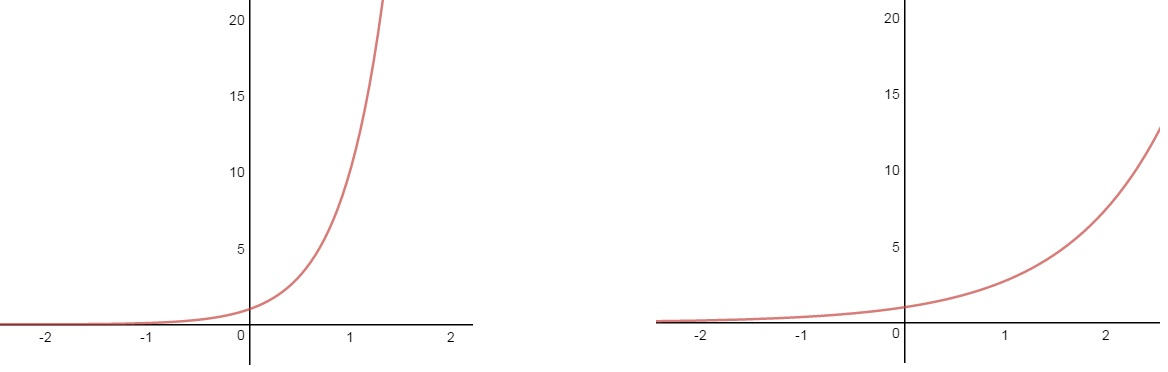
\includegraphics[width=6in]{Figures/exp10.jpg}
    \begin{solution}
      \(f^{-1}(15) \approx 1.2\), \(g^{-1}(5) \approx 1.6\)
    \end{solution}
    % Note to instructors: point out that they just estimated log(15)
    % and ln(5).  This is truly not obvious to them!
    \part The base-10 logarithm of $x$, written $\log_{10}(x)$ or just
    $\log(x)$, is the exponent we need to put on the 10 so that we get
    $x$.  That is, \(\log_{10}x = c\) means...
    \begin{solution}
     \(\log_{10}x = c\)  means \(10^c = x\).
    \end{solution}
    \vskip8ex
    \part The natural logarithm of $x$, written $\ln(x)$ is
    similar, except the base is $e$ instead. So, \(\ln(x) = c\) means..
    \begin{solution}
      \(\ln(x) = c\) means \(e^c = x\).
    \end{solution}
    \vskip8ex
    \part Estimate \(\log_{10}(15)\) and \(\ln(5)\).
    \begin{solution}
      By part (a), \(\log_{10}(15) \approx 1.2\) and \(\ln(5) \approx 1.6\).
    \end{solution}
  \end{parts}
  \question
  \begin{parts}
  \part What is $\log(1000)$?  $\log(1,000,000)$?  $\ln(e^{42})$?
    $\ln(1)$?

    \begin{solution}
     \(\log(1000) = 3\) since \(10^3 = 1000\). \(\log(1000000) = 6\)
     for similar reasons. \(\ln(e^{42}) = 42\). \(\ln(1) = 0\) since
     \(e^0 = 1\).
    \end{solution}

    \vskip5ex
	
	
  \part (1.4 \#45)
	
    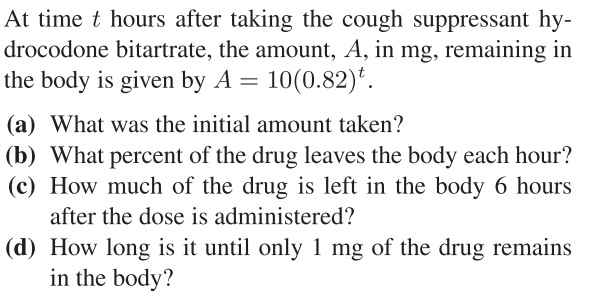
\includegraphics[width=4in]{Figures/no39.jpg}
    \begin{solution}
      \begin{enumerate}[(a)]
      \item The initial amount is \(10\)mg.
      \item The decay rate it \(1-0.82 = 0.18\). Therefore, \(18\%\)
        of the drug leaves the body each hour.
      \item \(A(6) = 10(0.82)^6\)mg. Note, this is approximately
        \(3.04\)mg, but you would want a calculator to compute this.
      \item We want to compute \(t\) such that \(10(0.82)^t = 1\). We check
        \begin{align*}
          10(0.82)^t = 1
          & \implies (0.82)^t = \frac{1}{10} \\
          & \implies \ln ((0.82)^t) = \ln(\frac{1}{10})\\
          & \implies t \ln(0.82) = \ln(0.1)\\
          & \implies t = \frac{\ln(0.1)}{\ln(0.82)} \text{ hours}
        \end{align*}
        Thus, there is only \(1\)mg of the drug in the body after
        \(\frac{\ln(0.1)}{\ln(0.82)} \text{ hours}\). We can use a
        calculator to compute
        this is \(11.6\) hours after taking the cough suppressant.
      \end{enumerate}
    \end{solution}
	\newpage
	\hspace*{-.6cm}\textbf{Note}: You should be comfortable using
        \textbf{all} the logarithm properties in the box on page 30.
	
	\vskip4ex
	
	
      \part Lily is studying a particular radioactive isotope of
        radon.  Ten minutes into her experiment, she measures that
        only 15\% of the radon remains.  Find the \textbf{half-life}
        of this isotope.\\ (You don't need any special formulas to do
        this!)
        \begin{solution}
          Let \(P(t)\) be the mass of the isotope after \(t\)
          minutes. We know that \(P(t) = P_0 a^t\) for some \(a\) and
          \(P_0\), so \(P(10) = P_0 a^{10}\). We also know that \(P(10) = 0.15 P_0\). Thus, we
          can combine our two formulas for \(P(10)\) 
          \begin{align*}
            P(10)/P(0) = \frac{P_0 a^{10}}{P_0 a^0} =
            \frac{0.15P_0}{P_0}
            & \implies a^{10} = 0.15 \\
            & \implies a = (0.15)^{\frac{1}{10}}
          \end{align*}
          Now, we want to know for which time \(t\) does \(P(t) =
          \frac{1}{2}P_0\). We compute
          \begin{align*}
            P_0 (0.15)^{\frac{t}{10}} = 0.5 P_0
            & \implies (0.15)^{\frac{t}{10}} = 0.5 \\
            & \implies \ln ((0.15)^{\frac{t}{10}}) = \ln(0.5) \\
            & \implies \frac{t}{10} \ln(0.15) = \ln(0.5)\\
            & \implies t = 10 \frac{\ln(0.5)}{\ln(0.15)} \text{ minutes}
          \end{align*}
        \end{solution}
        \vskip2in
      \part (1.4 \#55)

        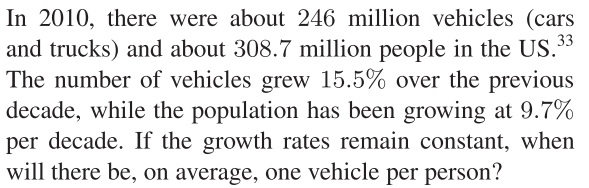
\includegraphics[width=4in]{Figures/no53.jpg}
        \begin{solution}
          Let \(V(t)\) be the number of cars in millions in the US \(t\) years after 2010
          and let \(P(t)\) be the number of people in millions in the US \(t\)
          years after 2010. From the statement of the problem, we know
          that the growth rate per decade, so to get the growth rate
          per year, we have to take the \(\frac{1}{10}\) power. Thus,
          we get \[
            V(t) = 246((1+0.155)^{\frac{1}{10}})^t =
            246(1.155)^{\frac{t}{10}}
            \]\[
            P(t) = 308.7((1+0.097)^{\frac{1}{10}})^t = 308.7(1.097)^{\frac{t}{10}}
          \]
          Now, we want to find \(t\) such that \(V(t) = P(t)\). We
          compute
          \begin{align*}
            V(t) = P(t)
            & \implies 246(1.155)^{\frac{t}{10}} =
                          308.7(1.097)^{\frac{t}{10}} \\
           & \implies \left( \frac{1.155}{1.097}
             \right)^{\frac{t}{10}} = \frac{308.7}{246}\\
           & \implies \ln\left(  \left( \frac{1.155}{1.097}
             \right)^{\frac{t}{10}} \right) = \ln\left(\frac{308.7}{246}\right)\\
           & \implies \frac{t}{10}\ln\left(   \frac{1.155}{1.097}
             \right)  = \ln\left(\frac{308.7}{246}\right)\\
           & \implies t 
             = 10 \ln\left(\frac{308.7}{246}\right) /
             \ln\left(   \frac{1.155}{1.097} \right) \text{ years}\\
          \end{align*}
          Thus, there will be, on average, one vehicle per person in \(10 \ln\left(\frac{308.7}{246}\right) /
             \ln\left(   \frac{1.155}{1.097} \right) \text{ years}\)
             after 2010.
          With a calculator, we can compute that this is approximately
          \(44.07\) years, so this will happen in \(2054\).
        \end{solution}
      \end{parts}
      \vspace{1.5in}
    \question Find the inverse of the function \(f(x) = 2^{3^x}\) and
    state its domain and range.
    \begin{solution}
      We wish to solve \(y = 2^{3^x}\) for \(x\). We compute
      \begin{align*}
        y = 2^{3^x}
        & \implies \ln(y) = \ln(2^{3^x}) \\
        & \implies \ln(y) = 3^x \ln(2) \\
        & \implies \frac{\ln(y)}{\ln(2)} = 3^x\\
        & \implies \ln \left(\frac{\ln(y)}{\ln(2)}  \right) = \ln(3^x)
        \\
        & \implies  \ln \left(\frac{\ln(y)}{\ln(2)}  \right) = x
          \ln(3)\\
        & \implies  x = \ln \left(\frac{\ln(y)}{\ln(2)}  \right)/\ln(3)
      \end{align*}
      Thus, \(f^{-1}(y) = \ln \left(\frac{\ln(y)}{\ln(2)}
      \right)/\ln(3)\). The domain of \(f^{-1}(y)\) is equal to the
      range of \(f(x)\), which is \((1,\infty)\) since \[
        0 < 3^x \implies 2^0 < 2^{3^x} \implies 1 < 2^{3^x} \,.
      \]
      The range of \(f^{-1}(y)\) is the domain of \(f(x)\) which is
      \((-\infty,\infty)\) since \(2^{3^x}\) is defined for all values
      of \(x\).
      % Since \(g(y) = \ln(y)\) has domain
      % \((0,\infty)\), it must be that \(f^{-1}(y)\) must have a domain
      % satisfying \(y > 0\) but also \[
      %   \frac{\ln(y)}{\ln(2)} > 0 \implies \ln(y) > 0 \implies
      %   e^{\ln(y)} > e^0 \implies y > 1.
      % \]
      % Thus, the domain of \(f^{-1}\) is \((1,\infty)\).
      % The range is \((-\infty, \infty)\)
    \end{solution}
    \vspace{0.75in}
    \question For each of the following functions, sketch its graph,
    and find the domain, range, and asymptotes (on a separate sheet of
    paper). \\
    (a) \(f(x) = 2^{-x+1}\), (b) \(f(x)=3+2^x\), (c) \(f(x) =
    \log_3(x-1)\), (d)  \(2-\log_2(x)\).
    \begin{solution}
      Check graphs with Desmos
% \begin{tikzpicture}
 
% \begin{axis}[
%     xmin = -1, xmax = 5,
%     ymin = -1.5, ymax = 4.0,
%     xtick distance = 1,
%     ytick distance = 1,
%     grid = both,
%     axis lines = middle,
%     minor tick num = 1,
%     major grid style = {lightgray},
%     minor grid style = {lightgray!25},
%     width = 0.5\textwidth,
%     height = 0.5\textwidth]
%     \addplot[
%         domain = -1:5,
%         samples = 200,
%         smooth,
%         thick,
%         blue,
%     ] {pow(2,-x+1) )};
% \end{axis}
% \end{tikzpicture}
(a) Domain: \((-\infty,\infty)\), range: \((0,\infty)\), asymptotes:
 \(y=0\).\\
(b) Domain: \((-\infty, \infty)\), range: \((3,\infty)\), asymptotes:
\(y=3\).\\
(c) Domain: \((1,\infty)\), range: \((-\infty,\infty)\), asymptotes:
\(x=1\).\\
(d) Domain: \((0,\infty)\), range: \((-\infty,\infty)\), asymptotes: \(x=0\).
    \end{solution}
    \vspace{0.2in}
    \question Solve each one of the following equations, showing every
    step of your work (on a separate sheet of paper).\\
    (a) \(3^{2x-7} = 27\), (b) \(5^{4-x} = \frac{1}{125}\), (c)
    \(3^{2x}-3^x-6 = 0\), (d) \(\log_2(5-x) + \log_2(5+x) = 4\).
    \end{questions}
    \begin{solution}
      Without work:
      (a) \(x=5\), (b) \(x=6\), (c) \(x=1\), (d) \(x = \pm 3\)\\
      Ask me if you need help solving.
    \end{solution}
  \end{document}
%%% Local Variables:
%%% mode: latex
%%% TeX-master: t
%%% End:
